% Generated by code/needham.py -- do not edit by hand.
\definecolor{qocA}{rgb}{0.00,0.45,0.70}
\definecolor{qocB}{rgb}{0.90,0.60,0.00}
\definecolor{qocC}{rgb}{0.00,0.62,0.45}
\definecolor{qocD}{rgb}{0.80,0.40,0.00}
\definecolor{qocE}{rgb}{0.80,0.60,0.70}
\definecolor{qocF}{rgb}{0.35,0.70,0.90}
\begin{tikzpicture}[ink/.style={line width=0.9pt, ndInk}, faint/.style={line width=0.4pt, ndInk!35}, dashedink/.style={line width=0.5pt, ndInk!55, dash pattern=on 2.5pt off 2pt}, vec/.style={->, >=stealth, line width=1.2pt}, note/.style={font=\footnotesize\itshape, text=ndInk!85, align=center}, pointer/.style={->, >=stealth, line width=0.4pt, ndInk!60, shorten >=2pt, shorten <=1pt}, dot/.style={circle, fill=ndInk, inner sep=0pt, minimum size=3.4pt}, wash/.style={fill=ndSky, fill opacity=0.55}, every node/.style={text=ndInk}]
\definecolor{ndInk}{rgb}{0.13,0.13,0.18}
\definecolor{ndPaper}{rgb}{0.99,0.96,0.88}
\definecolor{ndSky}{rgb}{0.84,0.91,0.98}
\definecolor{ndRose}{rgb}{0.98,0.86,0.84}
\definecolor{ndBlue}{rgb}{0.13,0.36,0.66}
\definecolor{ndRed}{rgb}{0.78,0.20,0.16}
\definecolor{ndGold}{rgb}{0.88,0.62,0.10}
\definecolor{ndGreen}{rgb}{0.18,0.52,0.30}
\fill[ndSky, fill opacity=0.5] (0,0) circle (2.500);
\draw[line width=1.6pt, ndBlue] (0,0) circle (2.500);
\draw[faint, ->, >=stealth] (-2.80,0) -- (3.00,0) node[below] {$x$};
\draw[faint, ->, >=stealth] (0,-2.80) -- (0,3.00) node[left] {$z$};
\node[dot, label={[font=\footnotesize]above right:$\ket0$}] at (0.000,2.500) {};
\node[dot, label={[font=\footnotesize]below right:$\ket1$}] at (0.000,-2.500) {};
\node[dot, label={[font=\footnotesize]above right:$\ket+$}] at (2.500,0.000) {};
\node[dot, label={[font=\footnotesize]left:$\ket-$}] at (-2.500,0.000) {};
\node[dot, fill=ndInk!60, label={[font=\footnotesize]below left:$\tfrac12\Id$}] at (0,0) {};
\draw[line width=1.1pt, ndRed] (0.439,2.461) -- (1.255,-2.162);
\node[dot, fill=ndRed] at (0.439,2.461) {};
\node[dot, fill=ndRed] at (1.255,-2.162) {};
\draw[line width=1.1pt, ndGreen] (2.182,1.221) -- (-2.456,-0.467);
\node[dot, fill=ndGreen] at (2.182,1.221) {};
\node[dot, fill=ndGreen] at (-2.456,-0.467) {};
\node[dot, minimum size=4.6pt, label={[font=\small]above left:$\rho$}] at (0.750,0.700) {};
\node[note, anchor=west] (n1) at (3.10,1.90) {pure states:\\ the sphere $\norm{\mathbf r}=1$};
\draw[pointer] (n1.west) to[bend right=15] (1.554,1.958);
\node[note, anchor=west] (n2) at (3.10,-0.40) {mixed states: inside;\\$\Tr\rho^2=\tfrac12(1+\norm{\mathbf r}^2)$};
\node[note, anchor=west] (n3) at (3.10,-2.30) {\textcolor{ndRed}{$\rho=0.62\,\rho_a+0.38\,\rho_b$}\\\textcolor{ndGreen!80!black}{$\rho=0.69\,\rho_{a'}+0.31\,\rho_{b'}$}\\same $\rho$, two different ensembles:\\ any chord through $\rho$ will do};
\draw[pointer] (n3.west) to[bend left=20] (0.850,0.625);
\node[above, font=\footnotesize] at (0.439,2.461) {$\rho_a$};
\node[below, font=\footnotesize] at (1.255,-2.162) {$\rho_b$};
\node[right, font=\footnotesize] at (2.182,1.221) {$\rho_{a'}$};
\node[left, font=\footnotesize] at (-2.456,-0.467) {$\rho_{b'}$};
\end{tikzpicture}
